\chapter{Marco  Teórico}

En el presente capítulo se introducen conceptos fundamentales relacionados al diseño inverso de dispositivos fotónicos.
Para ello se desarrolla seis secciones. 
Primero, se describen las propiedades físicas de interés de un \emph{bend} y WDM.
Segundo, se explica como parametrizar la región de diseño de estos
dispositivos.
Tercero, se detalla los pasos necesarios para poder simular computacionalmente
los diseños realizados.
Cuarto, se explica la estrategia de optimización a seguir con la
parametrización señalada.
Quinto, se describen tres algoritmos que se usaran en el presente trabajo: (i)
algoritmos genéticos (GA), (ii) \emph{particle swarm optimization} (CMA), (iii)
\emph{covariance matrix adaptation evolution strategy} (CMA-ES).
Finalmente, se expone que transformaciones se puede aplicar dentro de la
estrategia a seguir.

\leonidas{TODO: Actualizar esto al final.}

\section{Dispositivos de estudio}

\subsection{\emph{Bend}}

Un \emph{bend} es un dispositivo fotónico que se encarga de guiar el giro de un haz de ondas.

En general, al estudiar dispositivos fotónicos es de especial interés la
distribución del campo eléctrico ($\boldsymbol{E}$).
Este nos permite visualizar la distribución de la energía en un dispositivo calculando lo siguiente:

\begin{equation}
  |\boldsymbol{E}|^2 = |\boldsymbol{E_x}|^2+|\boldsymbol{E_y}|^2+|\boldsymbol{E_z}|^2,
\label{eq:field}
\end{equation}

donde $\boldsymbol{E_x}, \boldsymbol{E_y}, \boldsymbol{E_z}$ representan las componentes del campo eléctrico
en los ejes $x, y, z$, respectivamente
\citep{LukasChrostowski2010}.

\begin{figure}[ht]
  \centering
  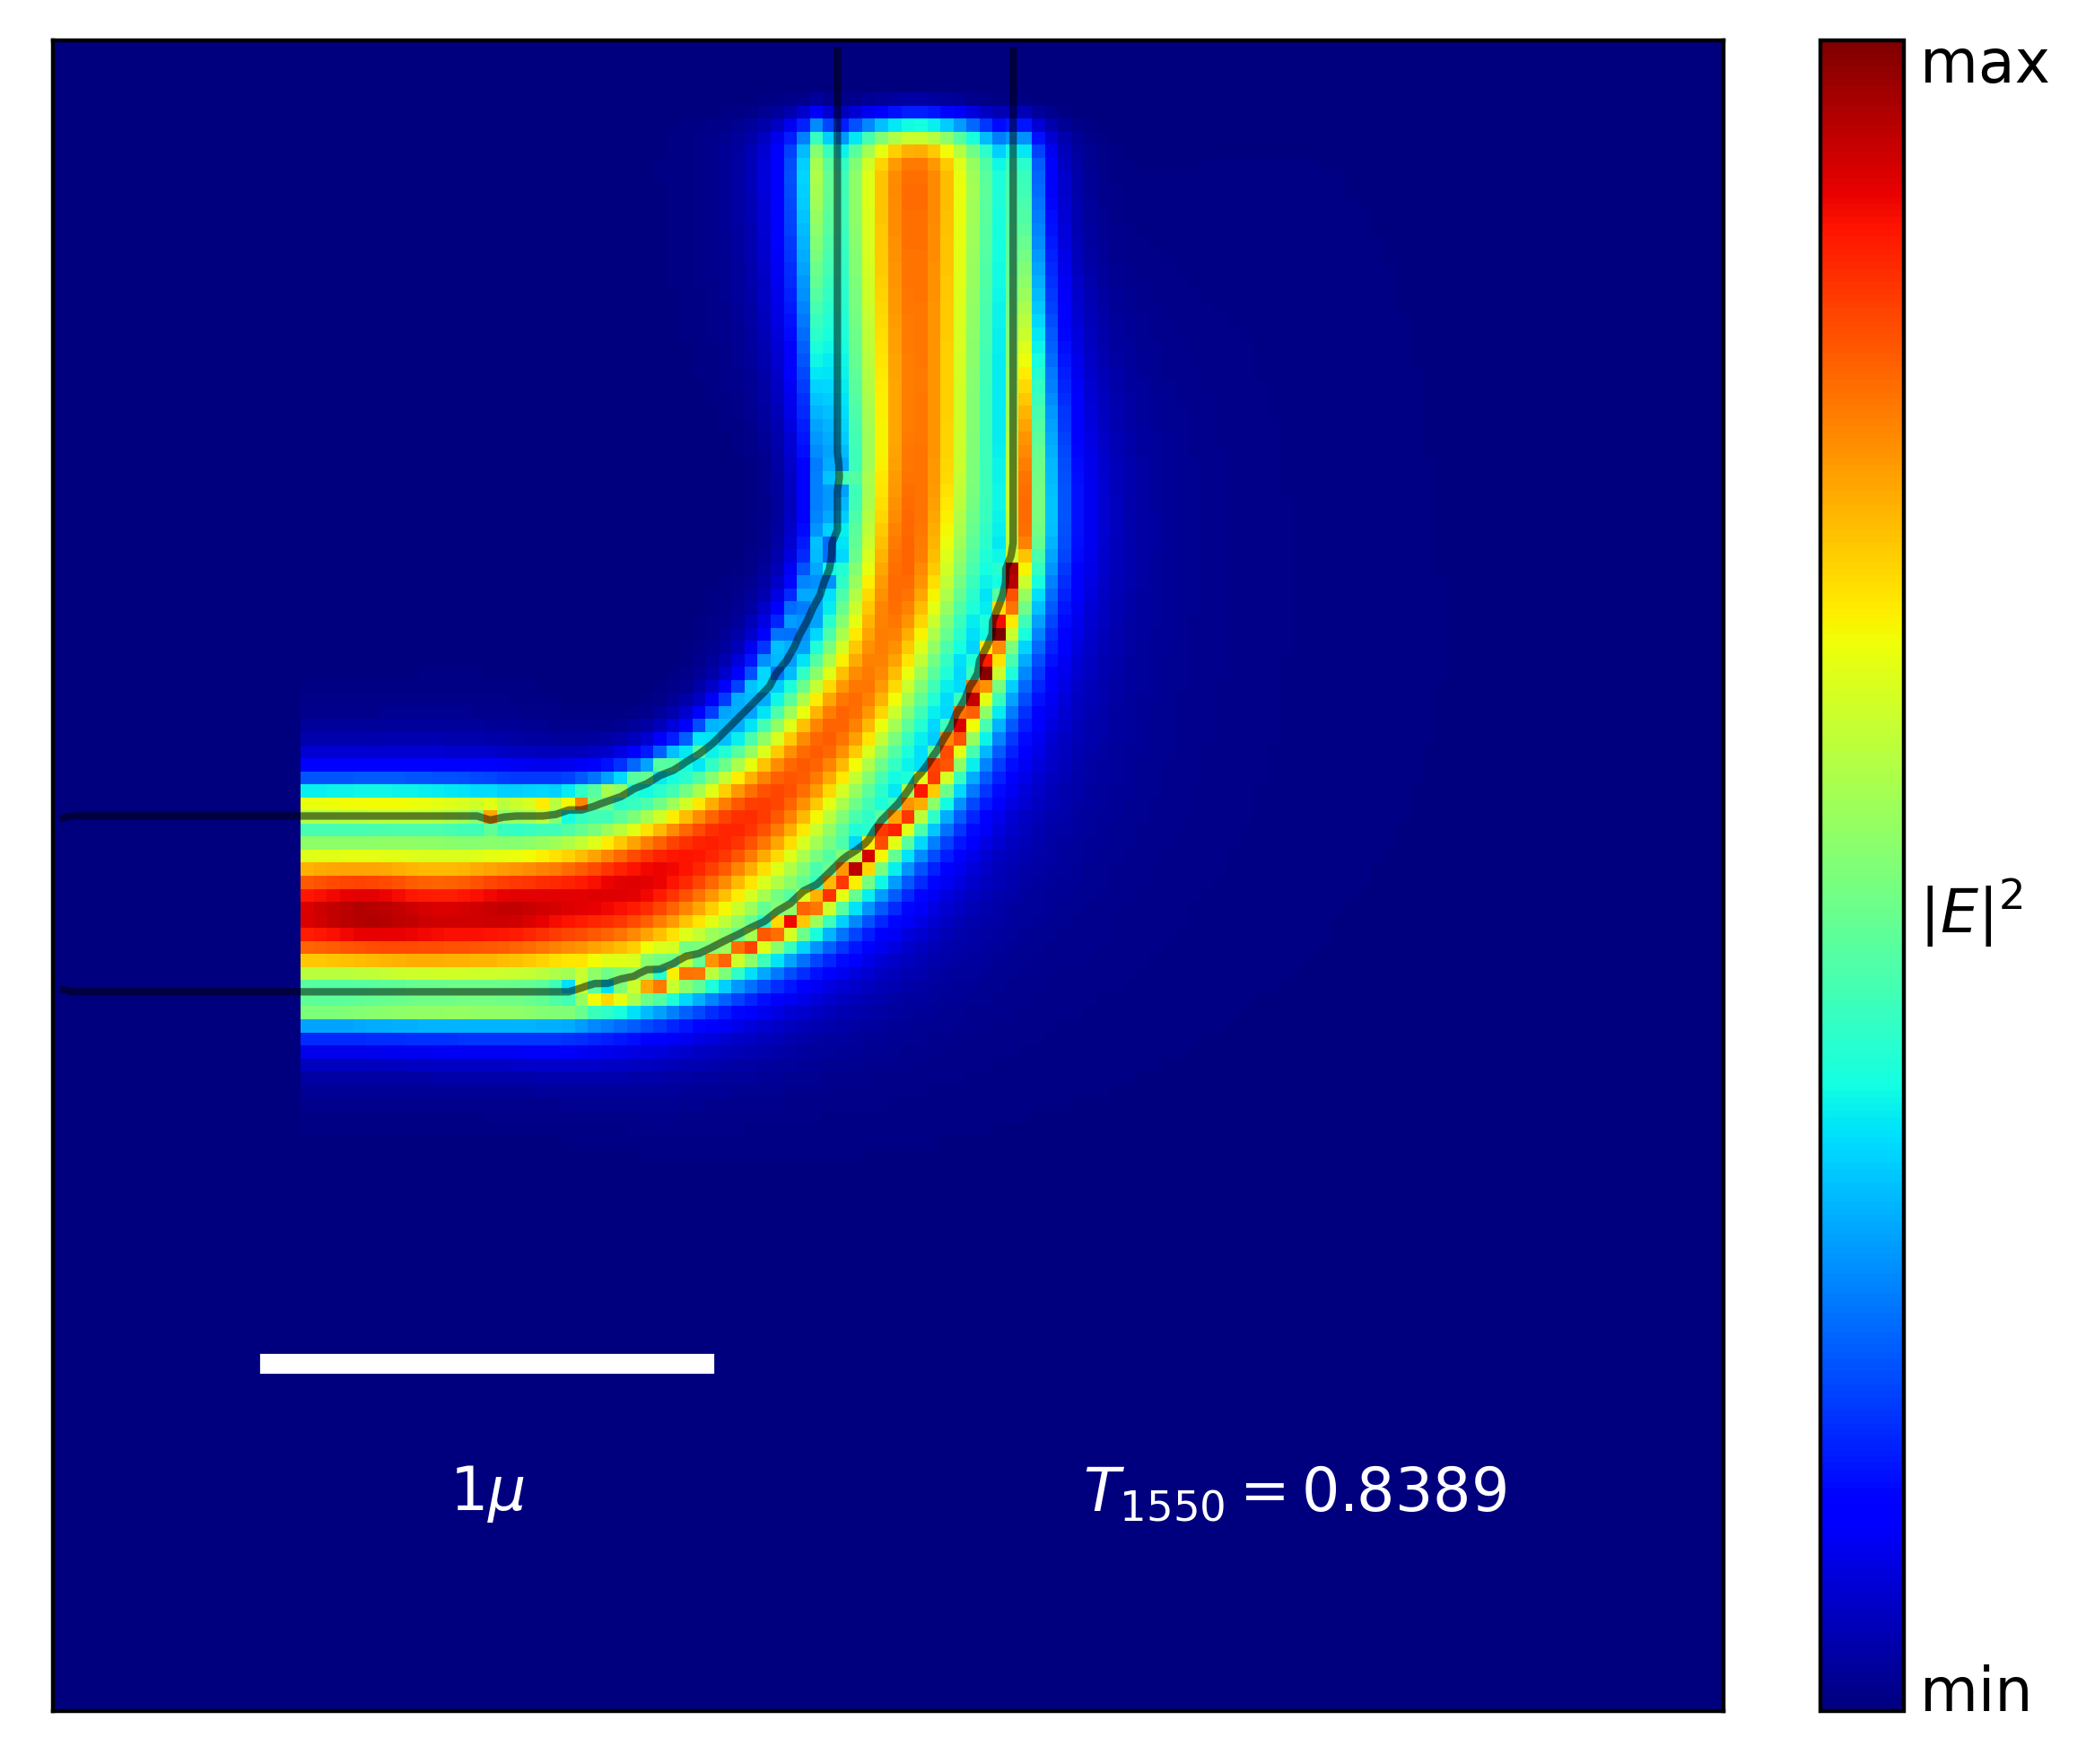
\includegraphics[scale=0.7]{image/theory/bend_field_dx30_px16_rint1000.png}
  \caption{Representación de $|\boldsymbol{E}|^2$ de un \emph{bend} de $1 \mu m$ de radio obtenido con una simulación en 3D FDFD con SPINS
  bajo una resolución de $30 nm$.}
  \label{fig:efield}
\end{figure}


Tradicionalmente, un \emph{bend} consiste en una una guía de onda horizontal usada como entrada y
una guía de onda vertical usada como salida, estas son conectadas por una guía de onda con la forma de un
cuarto de circunferencia de radio $r$ y con el mismo grosor de las guías de onda de entrada y salida.
En la \autoref{fig:efield} se muestra un \emph{bend} tradicional de radio $r = 1 \mu m$.
Como se observa en la imagen, parte significativa de la energía se pierde en la región curva.
Esto se debe a que el radio de curvatura es muy pequeño, con un valor más grande (e.g. $r = 10 \mu m$) 
las pérdidas se vuelven casi nulas \citep{LukasChrostowski2010}.


Para evitar ambigüedades, dos puntos adicionales a remarcar son: 
(i) cuando nos referimos al radio estamos haciendo mención al radio medio de curvatura y 
(ii) todos los diseños mostrados en este trabajo tienen un profundidad de 220nm.

Observar en una gráfica el valor de $|\boldsymbol{E}|^2$ nos ayuda a entender el funcionamiento de un dispositivo.
Por otro lado, una manera de cuantificar que tan bien funciona un diseño es mediante el cálculo de la
transmitancia $(T)$.
Este valor se define como la relación entre la potencia del flujo que sale del dispositivo con la 
potencia del flujo que ingresa \citep{Christiansen2021}.

Seguidamente, sea $\lambda$ la longitud de onda de la entrada y $\boldsymbol{P}$ los parámetros que caracterizan al
diseño, denotaremos como $T_{\lambda}(\boldsymbol{P})$ a la transmitancia asociada al dispositivo obtenido con la
parametrización $\boldsymbol{P}$ en la longitud de onda $\lambda$. Luego, definimos la función objetivo 
($f_{obj}$) para un \emph{bend}, también conocido en el área como figura de mérito (FOM), 
mediante la siguiente ecuación \citep{Su2020}:

\begin{equation}
  f_{obj}(\boldsymbol{P}) = max \left \{ T_{1550} (\boldsymbol{P}) \right \}.
\label{eq:fom-bend}
\end{equation}

En síntesis, la idea detrás de estas definiciones es describir un \emph{bend} mediante una parametrización
$\boldsymbol{P}$
(\autoref{sec:parametrization}).
Luego, usando algoritmos de optimización, buscar entre las distintas combinaciones de los parámetros aquella configuración
que optimice la función $f_{obj}$ (\autoref{sec:alg-opt}).
De este modo, estaremos encontrando un diseño con una elevada transmitancia, es decir con un buen desempeño.

\subsection{\emph{Wavelength Demultiplexer} (WDM)}

Un WDM es un dispositivo fotónico que se encarga de guiar un haz de ondas de acuerdo a su longitud de onda.
Por ejemplo, estos pueden trabajar con dos longitudes de onda y guían las de una longitud por la guía de onda superior
y las de otra longitud por la guía de onda inferior.

Análogo al caso del \emph{bend}, utilizaremos la transmitancia para cuantificar el desempeño del dispositivo.
Pero, en el presente trabajo usaremos un WDM con dos guías de salida, por ello, utilizaremos como notación
$T_{\lambda}^{(1)}(\boldsymbol{P})$ para
representar la transmitancia en la guía de salida superior cuando se recibe un haz de longitud de onda
$\lambda$ en un diseño descrito por los parámetros $\boldsymbol{P}$ y $T_{\lambda}^{(2)}(\boldsymbol{P})$ para la guía de salida inferior.

\begin{figure}[ht]
  \centering
  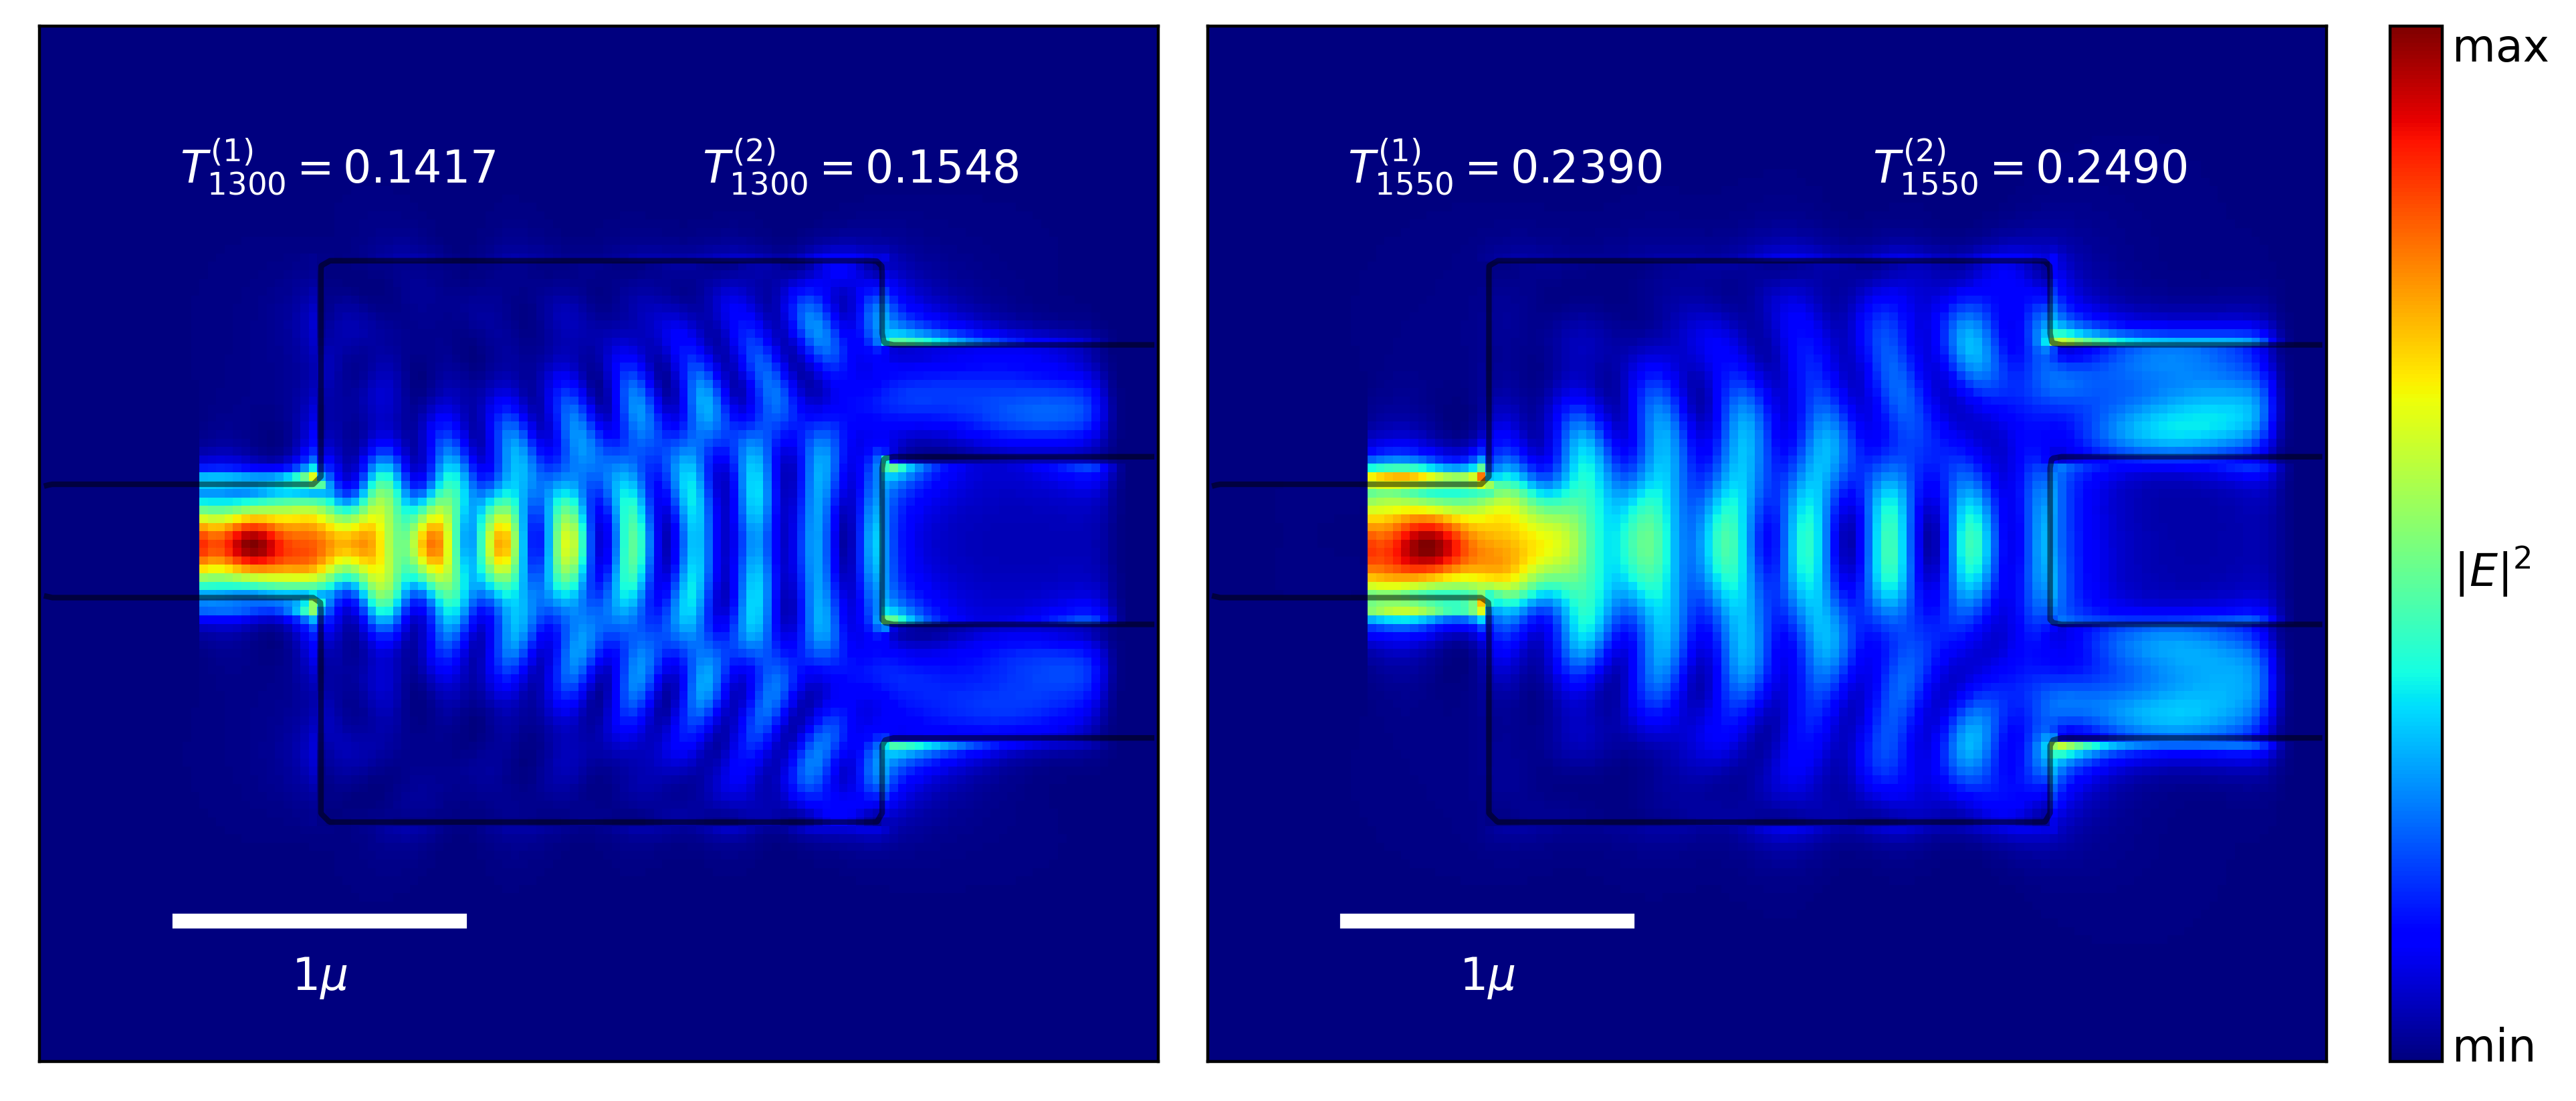
\includegraphics[scale=0.7]{image/theory/wdm_field_dx30_px16_px16.png}
  \caption{Representación de $|\boldsymbol{E}|^2$ de un WDM obtenido con una simulación en 3D FDFD con SPINS bajo una resolución de $30 nm$.}
  \label{fig:efield-wdm}
\end{figure}

En la \autoref{fig:efield-wdm} se muestra un WDM donde las guías de onda son unidas por una región rectangular
de $2.0\mu m \times 2.0 \mu m$. En el lado izquierdo se muestra la representación de $|\boldsymbol{E}|^2$ cuando se usa 
como entrada un haz de ondas de $1300 nm$ de longitud, en el lado derecho la entrada es de $1550 nm$.
En ambos casos el diseño está funcionando más como un \emph{splitter} que como un WDM.
Un \emph{splitter} es un dispositivo fotónico que divide la potencia del flujo de la entrada por las guías
de salida en una determinada proporción. El diseño intuitivo para este dispositivo es el presentado en la imagen. Similar al caso del
\emph{bend}, con unas dimensiones un poco más grandes se puede conseguir pérdidas casi nulas de energía
\citep{LukasChrostowski2010}.
Sin embargo, como se observa en los valores de la transmitancia, este diseño intuitivo no es apropiado para un WDM.

Basándonos en \cite{Su2020}, definimos su FOM como

\begin{equation}
  f_{obj}(\boldsymbol{P}) = max \left \{ \frac{\left ( T_{1300}^{(1)}(\boldsymbol{P}) \right )^2  + 
                            \left ( 1 - T_{1300}^{(2)}(\boldsymbol{P}) \right )^2 +
                            \left ( 1 - T_{1550}^{(1)}(\boldsymbol{P}) \right )^2  + 
                            \left ( T_{1550}^{(2)}(\boldsymbol{P}) \right )^2 }{4}
                    \right \}.
\label{eq:fom-splitter}
\end{equation}

La \autoref{eq:fom-splitter} busca maximizar la transmitancia por la guía de onda superior y minimizarla para
la guía de onda inferior cuando se recibe una longitud de onda de $1300 nm$ y lo contrario para una longitud
de onda de $1550 nm$. Cabe destacar que la división por cuatro se realiza para asegurar que $f_{obj}$ solamente
tenga valores en el intervalo $[0, 1]$, al igual que sucede con la función objetivo del \emph{bend}.

La idea para optimizar un WDM es la misma descrita en la anterior sección. 
En el resto del capítulo se describe en más detalle los otros pasos necesarios para lograr esto.

\section{Parametrización}\label{sec:parametrization}

Tanto para el \emph{bend} como para el WDM se define una región de diseño
mediante una parametrización ($\boldsymbol{P}$) que pueda mapear un gran conjunto de dispositivos.
Una de la estrategias más populares para esta tarea es usar parametrización
basada en píxeles, esta consiste en definir $\boldsymbol{P}$ como una matriz con valores en el intervalo
$[0, 1]$ \citep{Molesky2018}.

\begin{figure}[h]
  \centering
  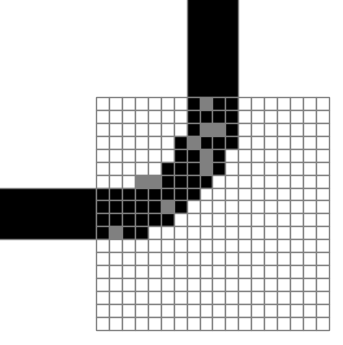
\includegraphics[scale=0.7]{image/theory/parametrization-pixeles.png}
  \caption{Parametrización basada en píxeles para un \emph{bend} definiendo $\boldsymbol{P}$ como una matriz de $18 \times 18$.}
  \label{fig:pixeles}
\end{figure}

Por ejemplo, en la \autoref{fig:pixeles} se ha definido la matriz $\boldsymbol{P}: [1, n] \times [1, m]
\to [0, 1]$ con $n = m = 18$ y se ha graficado sus valores
usando escala gris (0 corresponde al color blanco, 1 al negro y los demás valores a diferentes
intensidades del gris). De esta manera observamos como $\boldsymbol{P}$ logra definir la geometría de un
diseño.
Adicionalmente, conforme se incrementa el valor de $n, m$ se logra definir detalles con mayor precisión.


Sin embargo, lo anterior solo nos permite describir la geometría de los diseños, no sus propiedades.
Por ello, es necesario asociar a $\boldsymbol{P}$ alguna propiedad física.
Esto lo realizamos calculando la permitividad ($\varepsilon$) mediante la siguiente ecuación:

\begin{equation}
  \varepsilon(x, y) = \varepsilon_{Si} + (1 - p_{x,y})
  \varepsilon_{SiO_2} \, \mid \, x \in [1, n] \land y \in [1, m] \land p_{x,y} \in
  \boldsymbol{P},
\label{eq:permitivity}
\end{equation}

donde $\varepsilon_{Si} = 3.48$ es la permitividad del silicio ($Si$),
$\varepsilon_{SiO_2} = 1.44$ es la permitividad del óxido de silicio ($SiO2$) y $p_{x, y}$
es el elemento de $\boldsymbol{P}$ ubicado en la fila $x$, columna $y$.

Con la \autoref{eq:permitivity} estamos asociando a cada rectángulo de la geometría descrita por
$\boldsymbol{P}$ un valor de permitividad en el rango 
$[\varepsilon_{SiO2} = 1.44, 3.48 = \varepsilon_{Si}]$.
De esta manera, $p_{x, y} = 1$ describe que el rectángulo ubicado en la posición $(x, y)$ es de silicio,
un valor de $p_{x, y} = 0$ describe la presencia de óxido de silicio y $0 < p_{x, y} < 1$ hace referencia
a algún material cuya permitividad es $\varepsilon(x, y)$.

No obstante, un inconveniente de lo descrito es que $\boldsymbol{P}$ puede mapear a materiales inexistestes
(regiones grises),
en la \autoref{sec:estrategia-optimizacion} se estudia en más detalle esta dificultad.
Por otro lado, con la descripción de la permitividad ya podemos calcular los campos eléctricos con lo
cual se puede obtener el valor de $f_{obj}$ definido para el \emph{bend} y WDM.
Por tal motivo, se realiza una simulación electromagnética y se resuelve las inversas de las 
ecuaciones de Maxwell, esto permite obtener los campos eléctricos \citep{Su2020}.
Afortunadamente, para este proceso se puede utilizar distintos programas que utilizan diversos 
métodos numéricos para realizar los cálculos (\autoref{sec:simulation}).

\section{Simulación}\label{sec:simulation}

Una vez tenemos definido un dispositivo con regiones fijas (guías de onda) y una
región de diseño (descrita por la parametrización), es necesario incorporar
tres elementos adicionales \citep{Oskooi2010, Su2020}:

\begin{itemize}

  \item \textbf{Fuente:} Suele representarse como un rectángulo en un plano perpendicular al flujo
    que pasa por el lugar donde este se ubica. Simula la emición de un haz de ondas por el diseño.

  \item \textbf{Monitores:} Suelen representarse como un rectángulo similar a la fuente.
    Capturan información en su ubicación (e.g. valores del campo eléctrico).

  \item \textbf{PML:} Representan las condiciones de frontera en la simulación. 
    Se utilizan para limitar el espacio donde se deberá realizar las simulaciones computacionales.

\end{itemize}

\begin{figure}[ht]
  \centering
  \subfigure[Vista frontal]
    {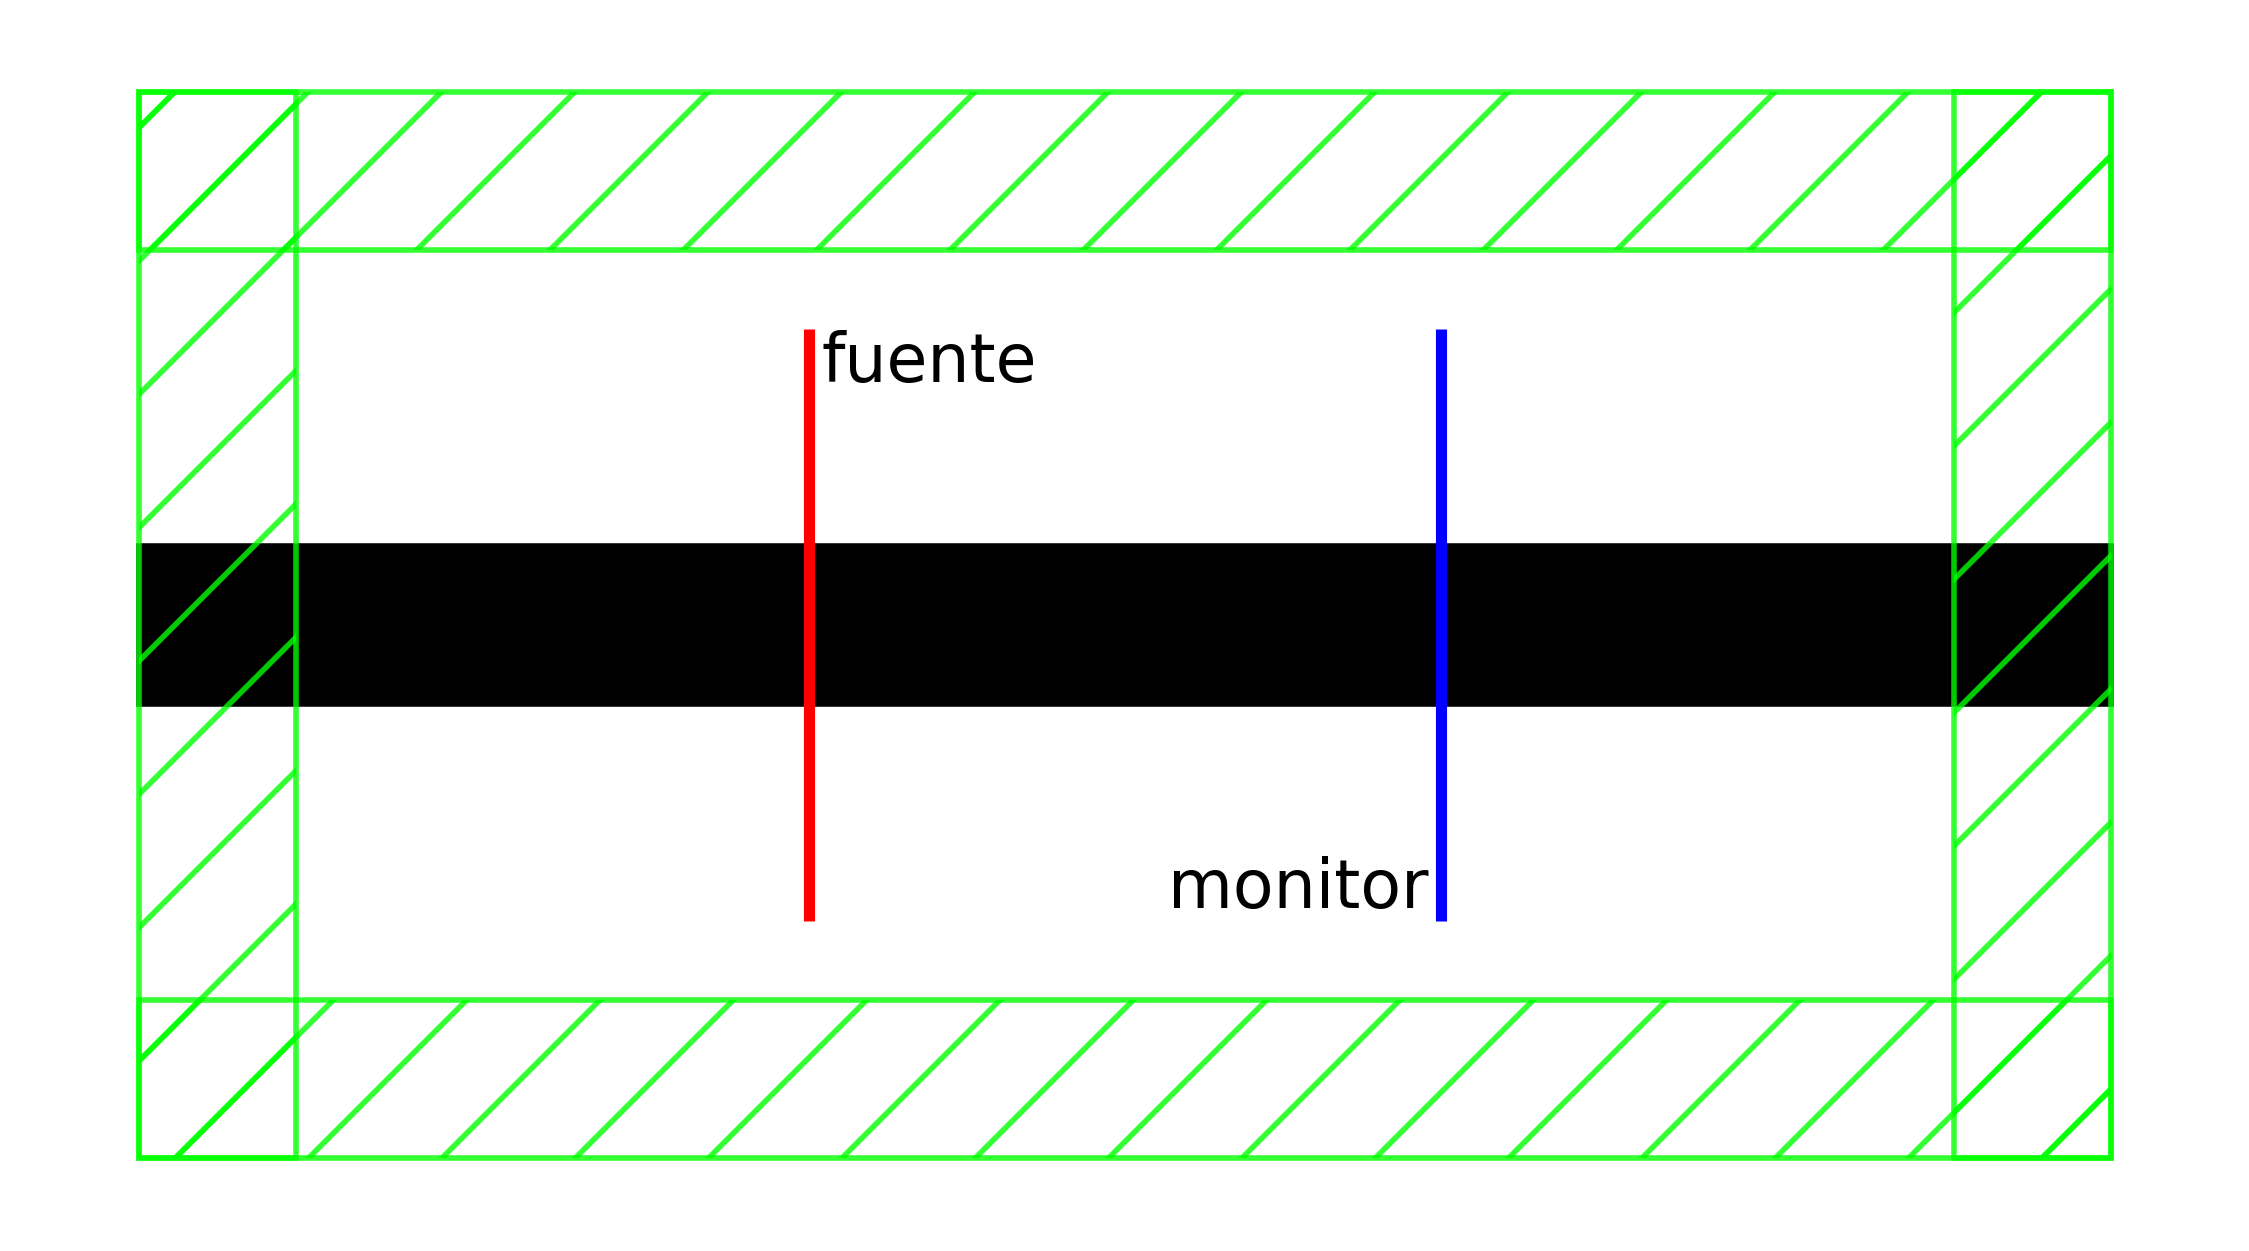
\includegraphics[width=0.45\textwidth]{image/theory/simulation.png}}
  \hfill
  \subfigure[Vista lateral]
    {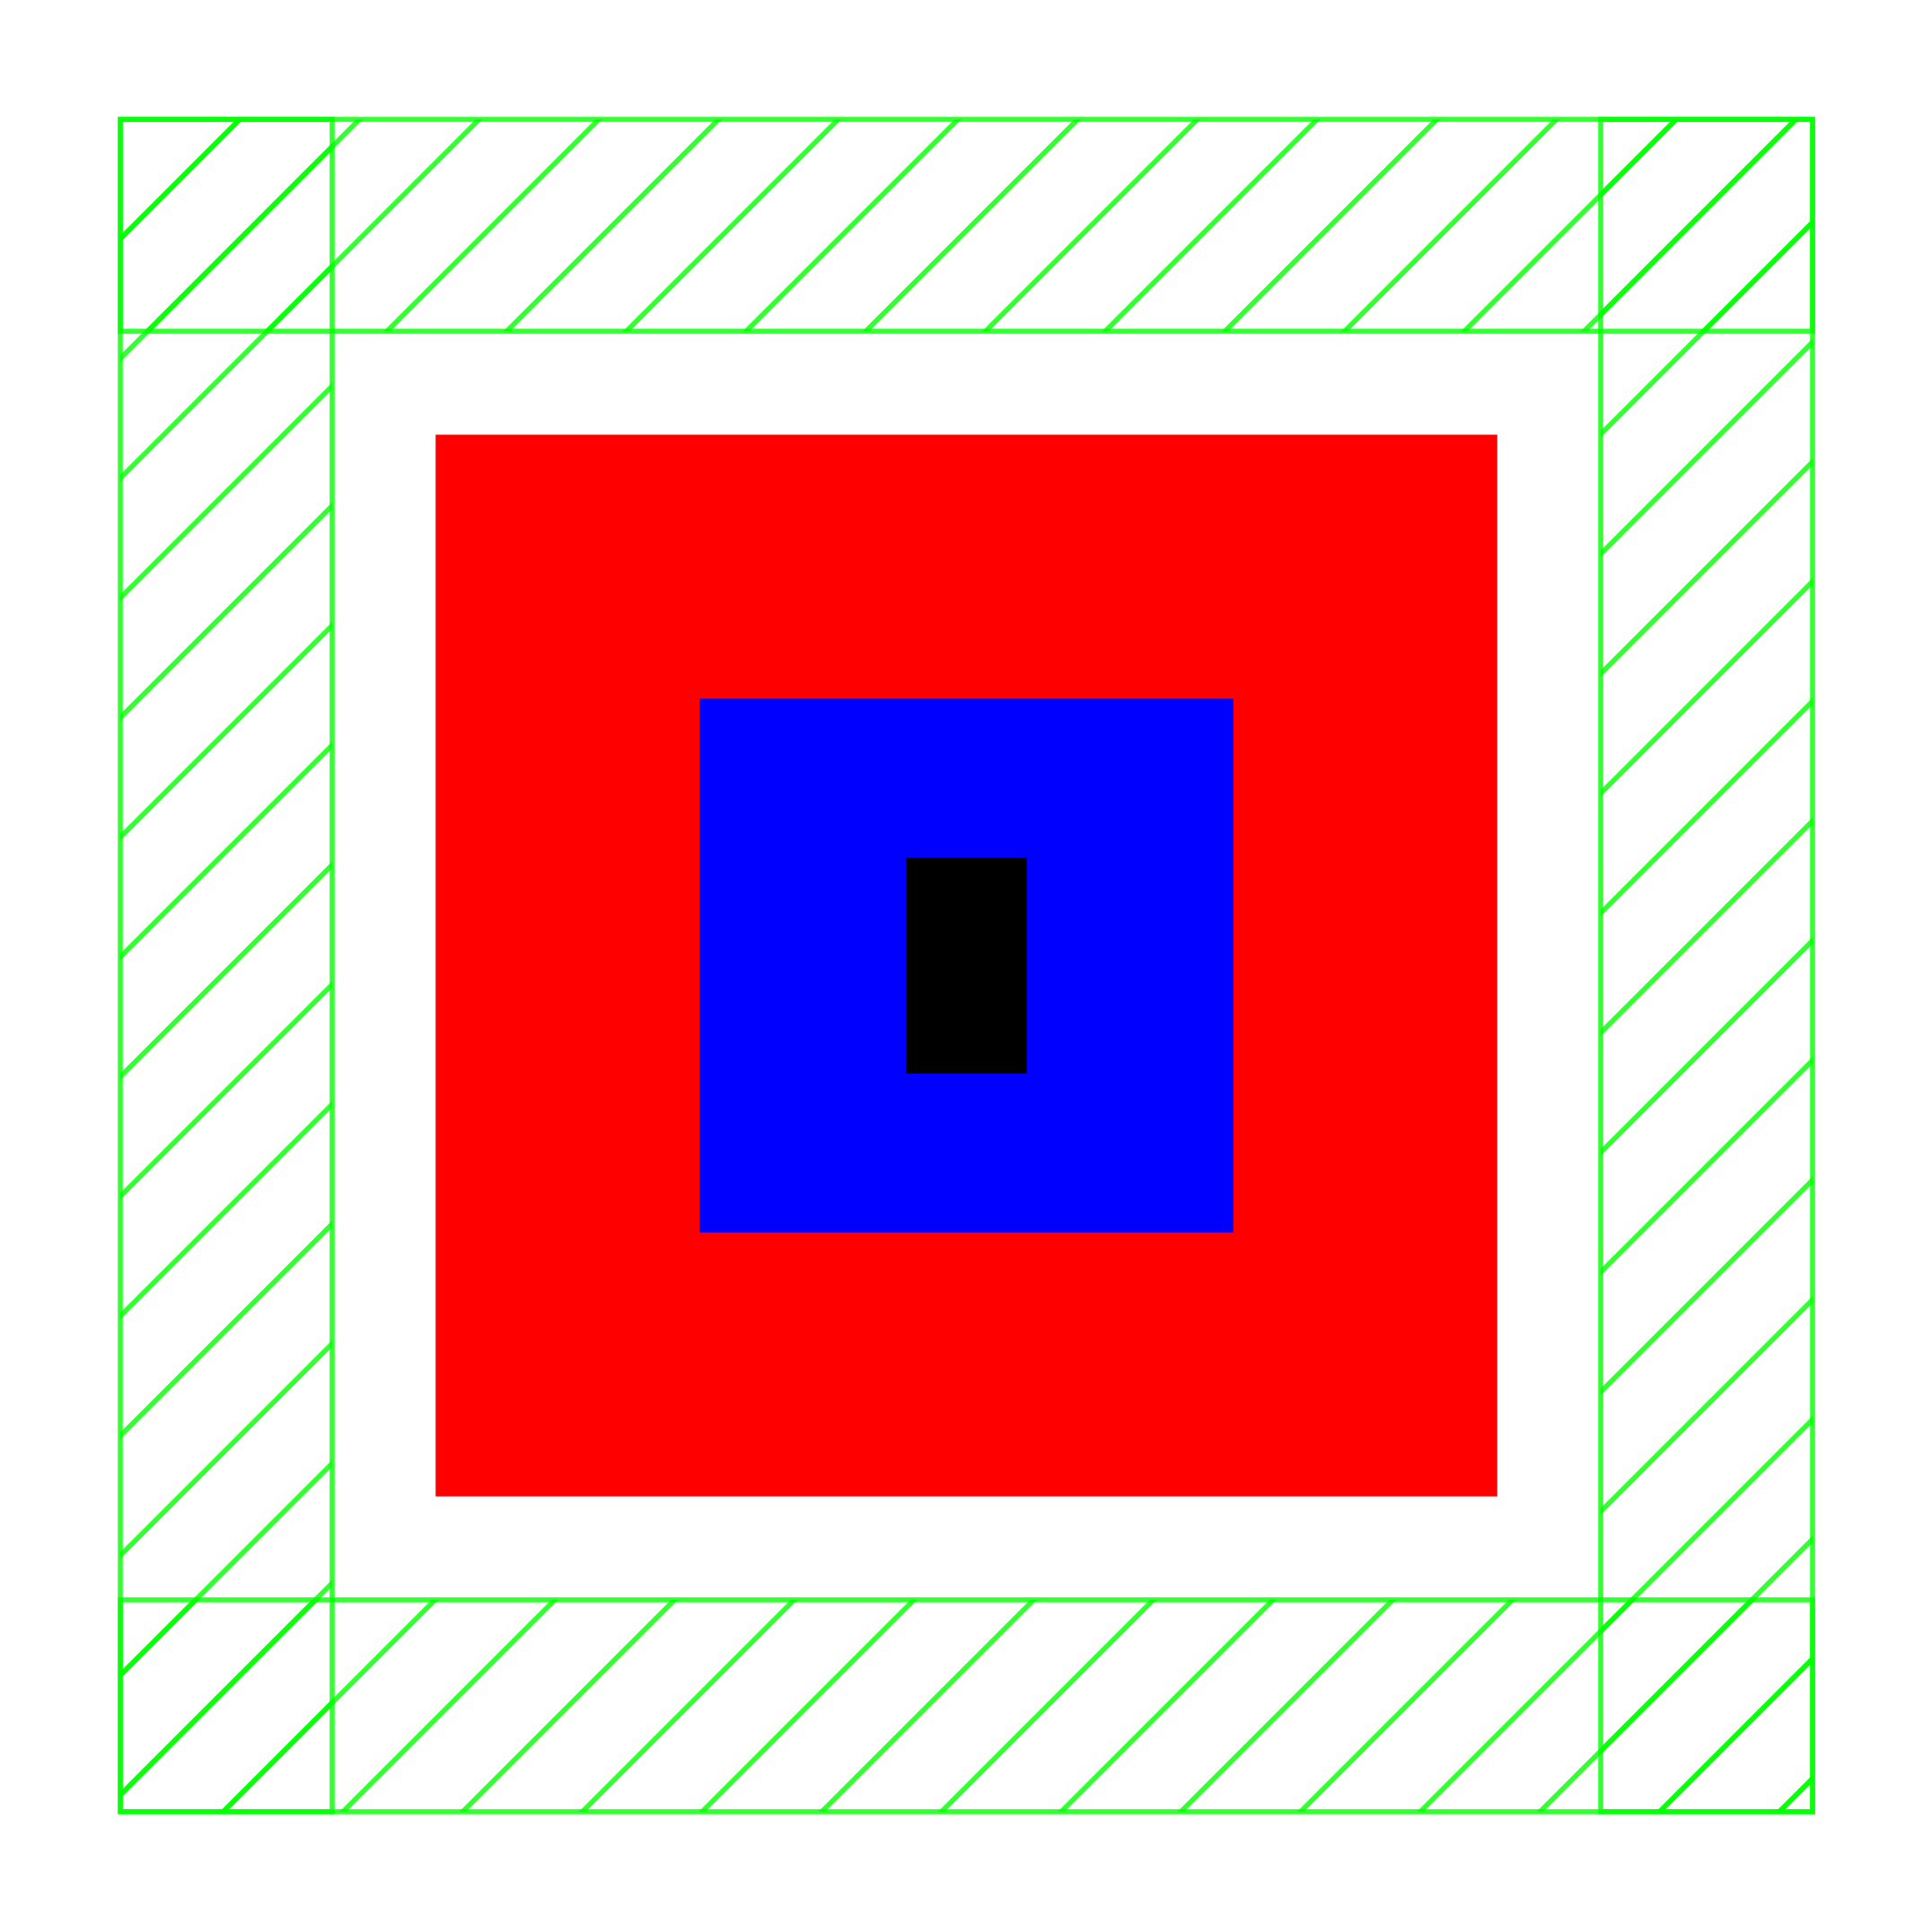
\includegraphics[width=0.45\textwidth]{image/theory/simulation-top.png}}

  \caption{Configuración de simulación para una guía de onda.}
  \label{fig:waveguide}
\end{figure}

En la \autoref{fig:waveguide} se ilustra una guía de onda con los elementos mencionados.
El rectángulo de color negro representa la guía de onda, la región roja la fuente, 
la región azul el monitor y lo verde el PML.
Guiándonos de la figura de la izquierda, al realizar una simulación con esta configuración 
el flujo iría de la región roja a la región azul.
Sin embargo, este seguiría expandiéndose por la guía de onda hasta llegar a la región verde (PML).
En palabras sencillas, podemos interpretar el PML como una caja que permite aislar nuestro sistema.
Por otro lado, la figura de la derecha representa el mismo diseño pero desde una vista lateral 
(recordemos que son diseños en 3D).
Aquí podemos evidenciar como la fuente y el monitor son representados por rectángulos, no por rectas.

Siguiendo lo descrito, para configurar y ejecutar simulaciones de un \emph{bend} y WDM podemos utilizar
diversos programas.
Dos librerías de Python de código abierto que permiten hacer estas tareas
son MEEP \citep{Oskooi2010} y SPINS \citep{Su2020}. 
Una evaluación cualitativa de sus funcionalidades puede ser observada en la \autoref{tab:simulation}.

\begin{table}[ht]
    \centering
    \begin{tabular}{|c|c|c|}
    \hline
    \textbf{Librería} & \textbf{MEEP} & \textbf{SPINS} \\
    \hline
    Usabilidad & Dificil & Moderada \\
    Eficiencia & Alta & Moderada-Alta \\
    Funcionalidad & Extensa & Básica-necesaria \\
    ¿Soporta GPU? & No & Sí \\
    ¿Implementa el método \emph{adjoint}? & Sí & Sí \\
    \hline 
    \end{tabular}
    \caption{Evaluación cualitativa de las librerías MEEP y SPINS.}
    \label{tab:simulation}
\end{table}

Como se describe en \autoref{tab:simulation}, desde mi punto de vista, MEEP es un programa eficiente y
con más funcionalidades que SPINS. Sin embargo, estas ventajas se reflejan en una usabilidad más
complicada. Además, en realidad, la eficiencia de SPINS es muy destacable en diversas situaciones,
en parte gracias a su implementación en GPU para las simulaciones. 
Finalmente, sobre el método \emph{adjoint} no hay inconvenientes en ninguno de los programas.
Este método permite calcular eficientemente (independientemente de la dimensión de $\boldsymbol{P}$) 
el valor de $\frac{\mathrm d f_{obj}(\boldsymbol{P})}{\mathrm d \boldsymbol{P}}$ \citep{Molesky2018}.

Por otro lado, ambas librerías utilizan métodos numéricos y permiten simulaciones en 1D, 2D y 3D.
Particularmente, podemos definir un parámetro $dx$ para discretizar nuestro espacio de
simulación en una malla de cuadrados de dimensiones $dx \times dx$.
En general, cuanto más pequeño sea este valor
los resultados serán más precisos, pero la cantidad de memoría y el tiempo de
simulación se incrementarán considerablemente.
Es importante señalar que debemos procurar trabajar con un valor de $dx$ menor a las dimensiones
de nuestros rectángulos de la parametrización para poder simular nuestras geometrías con mejor
precisión.


Adicionalmente, mientras MEEP utiliza un método conocido como FDTD para las simulaciones,
SPINS usa FDFD. Por un lado, MEEP permite calcular la función objetivo en un rango de longitudes
de onda usando una sola simulación. En cambio, para realizar esta tarea SPINS debe realizar una simulación
por cada longitud de onda.

\section{Estrategia de optimización}\label{sec:estrategia-optimizacion}

Como fue descrito en la \autoref{sec:parametrization}, podemos
tener diseños que no puedan ser fabricados.
Para evitar esto se necesita obtener que $p_{x, y}$ de la \autoref{eq:permitivity} tenga valores enteros.
Sin embargo, al optimizar la función $f_{obj}$ no podemos asegurar esta condición.
Ante esta dificultad, \cite{Su2020} trabaja en dos etapas:


\begin{enumerate}

\item{\textbf{Optimización continua}}

En esta etapa se optimiza la función $f_{obj}$ sin imponer ninguna restricción.
    En la \autoref{sec:alg-opt} se detalla algoritmos que suelen usarse para este fin.

\item{\textbf{Optimización discreta}}

Se utiliza el resultado de la optimización continua como punto inicial para el algoritmo de optimización que se escoja.
Luego, se trabaja por iteraciones.
En cada iteración se aplica una transformación a cada diseño antes de evaluar su FOM.
Esta transformación se escoge de tal manera que ayude a ir convergiendo a un diseño fabricable, es decir,
a tener $p_{x, y} = 0$ o $p_{x, y} = 1$, más detalles en la \autoref{sec:transformations}.
Así, la idea de realizarlo por iteraciones es ir discretizando nuestro diseño
de forma suave e intentando mantener un buen valor del FOM.
Por ello, es crucial utilizar el resultado de una iteración como punto inicial de la próxima.

\end{enumerate}

\section{Algoritmos de Optimización}\label{sec:alg-opt}

Como observamos en la anterior sección, es necesario escoger algún algoritmo
que nos permita optimizar la función $f_{obj}$. 
Por este motivo, se presentan los siguientes tres algoritmos que serán usados en el presente trabajo.

\subsection{\emph{Genetic Algorithms} (GA)}

\leonidas{TODO: Actualizar nomenclatura.}

Como se describe en el Algoritmo \ref{alg:GA} \citep{Mykel2019}, la idea es  
comenzar generando una población (\emph{population}) de $n$ individuos representados por $p$
parámetros, línea 1. 
Los siguientes tres pasos se ejecutan por $k$ iteraciones.
Primero, se realiza un proceso de selección para obtener los mejores individuos
(\emph{parents}), línea 3.
Segundo, los seleccionados se encargan de producir la nueva generación
(\emph{children}), línea 4.
Tercero, la nueva generación muta obteniendo nuevas características, línea 5.

\begin{algorithm}
%\footnotesize
$population = generate\_population(n, p)$ \\
\For{$t = 0; \, t < k; \, t$++}{
    $parents = select(population)$ \\
    $children = crossover(population, parents)$ \\
    $population = mutation(children)$
}
\caption{Estructura de un algoritmo genético}
\label{alg:GA}
\end{algorithm}

Entrando en más detalle, para nuestro caso tenemos:

\begin{itemize}
    \item $generate\_population(n, p):$ retorna $n$ vectores de dimensión $p$
      con valores aleatorios en $U(0, 1)$.

    \item $select(population):$ retorna $number\_selected\_GA$ individuos de
      acuerdo a la probabilidad $prob_i$ dada por la ecuación
    
    \begin{equation}
      prob_i = \frac{f_{obj}^{(i)} - min(f_{obj})}{\displaystyle\sum_{j} (f_{obj}^{(j)} - min(f_{obj}))},
    \label{eq:prob}
    \end{equation}
    
    donde $f_{obj}^{(i)}$ está asociado con el $i-$ésimo individuo.
    
    \item $crossover(population, parents):$ retorna $n$ vectores de dimensión $p$.
    El $i-$ésimo vector es la combinación de dos padres aleatorios $pa_i$
    y $pb_i$ seleccionados de $parents$ y su $j-$ésimo parámetro es escogido
    con igual probabilidad entre el $j-$ésimo parámetro de $parents[pa_i]$
    y $parents[pb_i]$.

    \item $mutation(children):$ retorna lo que recibe, pero a cada atributo de
      cada individuo se le agrega un valor en $U(-range\_GA, range\_GA)$ con
      probabilidad de 0.5.

\end{itemize}

\subsection{\emph{Gradient Genetic Algorithms} (G-GA)}

\leonidas{TODO: Completar esto}

\subsection{\emph{Particle Swarm Optimization} (PSO)}

\leonidas{TODO: Actualizar nomenclatura.}

Podemos pensar este algoritmo como un caso especial del Algoritmo \ref{alg:GA}
\citep{Mykel2019, Prosopio-Galarza2019}.
La idea es visualizar el $i-$ésimo individuo como una partícula definida por: 
(i) su posición $x^{(i)}$ (el vector $p$-dimensional asociado al $i-$ésimo individuo),
(ii) su velocidad $\nu^{(i)}$ (un número real) y
(iii) la mejor posición encontrada hasta el momento.

Cada particula acumula velocidad en una dirección favorable dada por: 
(i) la mejor posición encontrada hasta el momento por ella y 
(ii) la mejor posición encontrada por la población completa.
Como consecuencia, los individuos se pueden mover independientemente de
perturbaciones locales.
Adicionalmente, agregando caminos aleatorios las particulas incorporan
comportamientos impredecibles que puede permitirles encontrar potenciales
mejores direcciones.

Entrando en más detalle, siguiendo la estructura del Algoritmo \ref{alg:GA}, tenemos:

\begin{itemize}

\item $generate\_population(n, p):$ retorna $n$ particulas con cada uno de
      sus parámetros tomando valores aleatorios en $U(0, 1)$.

\item $select(population):$ retorna la particula con el mejor $f_{obj}$

\item $crossover(population, parents):$ retorna la población luego de aplicar 
    
  \begin{equation}
    x^{(i)} \gets x^{(i)} + \nu^{(i)},
  \label{pso-pos}
  \end{equation}

  \begin{equation}
    \nu^{(i)} \gets \omega \nu^{(i)} + c_1 r_1 \left(x_{b}^{(i)} - x^{(i)}
    \right) + c_2 r_2 \left(x_{b} - x^{(i)} \right),
  \label{pso-speed}
  \end{equation}
    

  donde $x_{b}$  es la mejor posición encontrada globalmente, 
  $\omega$ representa la tendencia de la particula de conservar su velocidad actual,
  $c_1$ y $c_2$ cuantifica la atracción relativa de $x_{b}^{(i)}$ y $x_{b}$ respectivamente, 
  y $r_1, r_2 \in U(0, 1)$ representan el comportamiento impredecible.

\end{itemize}

\subsection{\emph{Gradient Particle Swarm Optimization} (G-PSO)}

\leonidas{TODO: Completar esto}

\subsection{\emph{Covariance Matrix Adapatation Evolution Strategy} (CMA-ES)}

\leonidas{TODO: Actualizar nomenclatura.}

La idea general de esta estrategia evolutiva, mostrada en el Algoritmo
\ref{alg:CMA}, es mantener:
(i) un vector $\mu$ $p$-dimensional,
(ii) una matriz $\Sigma$ y
(iii) un número $\sigma$ para ir generando $n$ inviduos $p$-dimensionales
a partir una distribución $\mathcal{N}(\mu,\,\sigma^{2} \Sigma)$.


Tomar puntos de esta distribución limita el espacio de búsqueda a una
hiperelipse.
Luego, el algoritmo evalua puntos en esta región limitada.
Usando los valores obtenidos, se puede decidir entre:
(i) mover la hiperelipse a otra región del espacio de búsqueda
(ii) expandir or reducir la región cubierta por la distribución.
El algoritmo de CMA-ES trabaja iterativamente sobre esta idea hasta que la
hiperelipse termina casi degenerándose en un punto, 
potencialmente un óptimo.
Para una descripción más detallada del algoritmo, revisar \citep{Mykel2019, Hansen2016}.

\begin{algorithm}
%\footnotesize
\For{$t = 0; \, t < k; \, t$++}{
    sample() \tcp{Obtener $n$ puntos de $\mathcal{N}(\mu,\,\sigma^{2} \Sigma)$}
    update() \tcp{Ecuación \ref{cma-average}}
    control() \tcp{Ecuación \ref{cma-control}}
    adapt() \tcp{Ecuación \ref{cma-adapt}}
}
\caption{CMA-ES}
\label{alg:CMA}
\end{algorithm}

Entrando en más detalle del Algoritmo \ref{alg:CMA} y considerando variables
globales por simplicidad, podemos resumir el procedimiento en cinco pasos.
En la línea 1 simplemente se repite las siguientes líneas por $k$ iteraciones.
En la iteración $t$, comenzamos con la línea 2 generando $n$ puntos
$p$-dimensionales $x_i$ de la distribución $\mathcal{N}(\mu,\,\sigma^{2} \Sigma)$, 
donde estos son ordenados descendentemente de acuerdo
al valor de $f_{obj}$.
En la línea 3 actualizamos la media $\mu$ usando una promedio ponderado dado
por

\begin{equation}
    \mu^{(t + 1)} \gets \sum_{i=1}^{n} w_i x_i,
\label{cma-average}
\end{equation},

donde $w_i$ son fijos y escogidos de tal manera que proporcionen mayor
contribución a los puntos con meyor $f_{obj}$. Esto permite mover la media $\mu$
en una dirección favorable.

Seguidamente, se necesita actualizar $\sigma$ para expandir o reducir la
hiperelipse en la siguiente iteración. Por este motivo, la línea 4 controla
este valor mediante las ecuaciones

\begin{equation}
    \sigma^{(t + 1)} \gets \sigma^{(t)} \exp\bigg(\frac{c_{\sigma}}{d_{\sigma}}
    \underbrace{\left(\frac{||p_{\sigma}||}{\mathbb{E}||\mathcal{N}(0,
    \mathbf{I})||} - 1 \right)}_{\text{evolution path comparison}} \bigg),
\label{cma-control}
\end{equation}

\begin{equation}
\mathbb{E}||\mathcal{N}(0, \mathbf{I})|| = \sqrt{2} \left(
  \frac{\Gamma\left(\frac{p + 1}{2}\right)}{\Gamma\left({\frac{p}{2}}\right)}
  \right),
\label{cma-E}
\end{equation}

donde $p_{\sigma}$ es una variable que acumula los pasos llevados,
$c_{\sigma} \in [0, 1]$ es una variable que determina el tiempo acumulado para $p_{\sigma}$ y 
$d_{\sigma} \approx 1$ es un parámetro que determina el ratio de posibilidad de cambio de $\sigma^{(t + 1)}$. 
La principal parte de la \autoref{cma-control} es el término \emph{evolution path comparison}, 
aquí se compara el tamaño de $p_{\sigma}$ con su tamaño esperado bajo selección
aleatoria.
De esta comparación podemos controlar si el valor de $\sigma$ debe
incrementarse, disminuirse o permanecer igual.

Finalmente, en la línea 5 cambiamos $\Sigma$ a una dirección favorable usando

\begin{multline}
    \Sigma^{(t + 1)} \gets \overbrace{\bigg(1 - c_1 c_c (1 - h_{\sigma})(2 - c_c) - c_1 - c_{\mu}\bigg) \Sigma^{(t)}}^{\text{cumulative update}} \\
    + \underbrace{c_{1} p_{\Sigma} p_{\Sigma}^{T}}_{\text{rank-one update}}
    + \underbrace{c_{\mu}\sum_{i=1}^{n}w'_{i}
    \delta^{(i)}\left(\delta^{(i)}\right)^{T}}_{\text{rank-}\mu\text{ update}},
\label{cma-adapt}
\end{multline}

donde $c_{\mu} \leq 1$ es el radio de aprendizaje para el término \emph{rank-$\mu$ update}, 
$c_1 \leq 1 - c_{\mu}$ es el radio de aprendizaje para el término \emph{rank-one update}, 
$c_c \in [0, 1]$ es el radio de aprendizaje para el término \emph{cumulative update}, 
$h_{\sigma}$ es la evaluación bajo la función unitaria usado para actualizar
apropiadamente el camino evolutivo, 
$p_{\Sigma}$ es un vector acumulativo usado para actualizar la matriz de
covarianza, 
$w'_i$ son los coeficientes de ponderación modificados y
$\delta^{(i)}$ son las desviaciones seleccionadas.

En la \autoref{cma-adapt}, el primer término (\emph{cumulative update}) 
mantiene información de la anterior matriz de convarianza.
El segundo término (\emph{rank-one update}) permite expandir la distribución en
una dirección favorable.
El tercer término (\emph{rank-$\mu$ update}) incrementa la búsqueda en espacios
donde es probable encontrar buenas soluciones.
La combinación de estos tres términos actualiza $\Sigma$ de tal manera que
mueva la hiperelipse en una dirección favorable.

\subsection{\emph{Gradient Covariance Matrix Adapatation Evolution Strategy} (G-CMA-ES)}

\leonidas{TODO: Completar esto}

\subsection{L-BFGS-B}

\leonidas{TODO: Completar esto}

\subsection{MMA}

\leonidas{TODO: Completar esto}

\section{Transformaciones}\label{sec:transformations}

La aplicación de transformaciones a un diseño se realiza con el fin de obtener
dispositivos que se puedan fabricar con mayor facilidad \citep{Su2020}. 

Basándonos en \cite{Zhang2021}, una manera de asegurar que los
parámetros $p$ describan un diseño más fácil de fabricar es aplicacando la función $s(p)$
descrita como

\begin{equation}
  \widetilde{\widetilde{\boldsymbol{P}}}(x, y) = \frac{\tanh (\beta \times \eta) + \tanh (\beta \times (p_{x, y}
  - \eta))}{\tanh (\beta \times \eta) + \tanh (\beta \times (1 - \eta))},
  \label{eq:projection}
\end{equation}

    donde $\eta = 0.5$ y $\beta$ comienza con un valor de 1 y va incrementándose exponencialmente en cada iteración. 
    Como se observa en la \autoref{fig:discretization}, la \autoref{eq:projection} se encarga de ir haciendo converger los valores de la parametrización a $0$ o $1$ de acuerdo a cual esté más cercano. 
    Conforme aumenta el valor de $\beta$ esta convergencia es más rápida.

    \begin{figure}[ht]
      \centering
      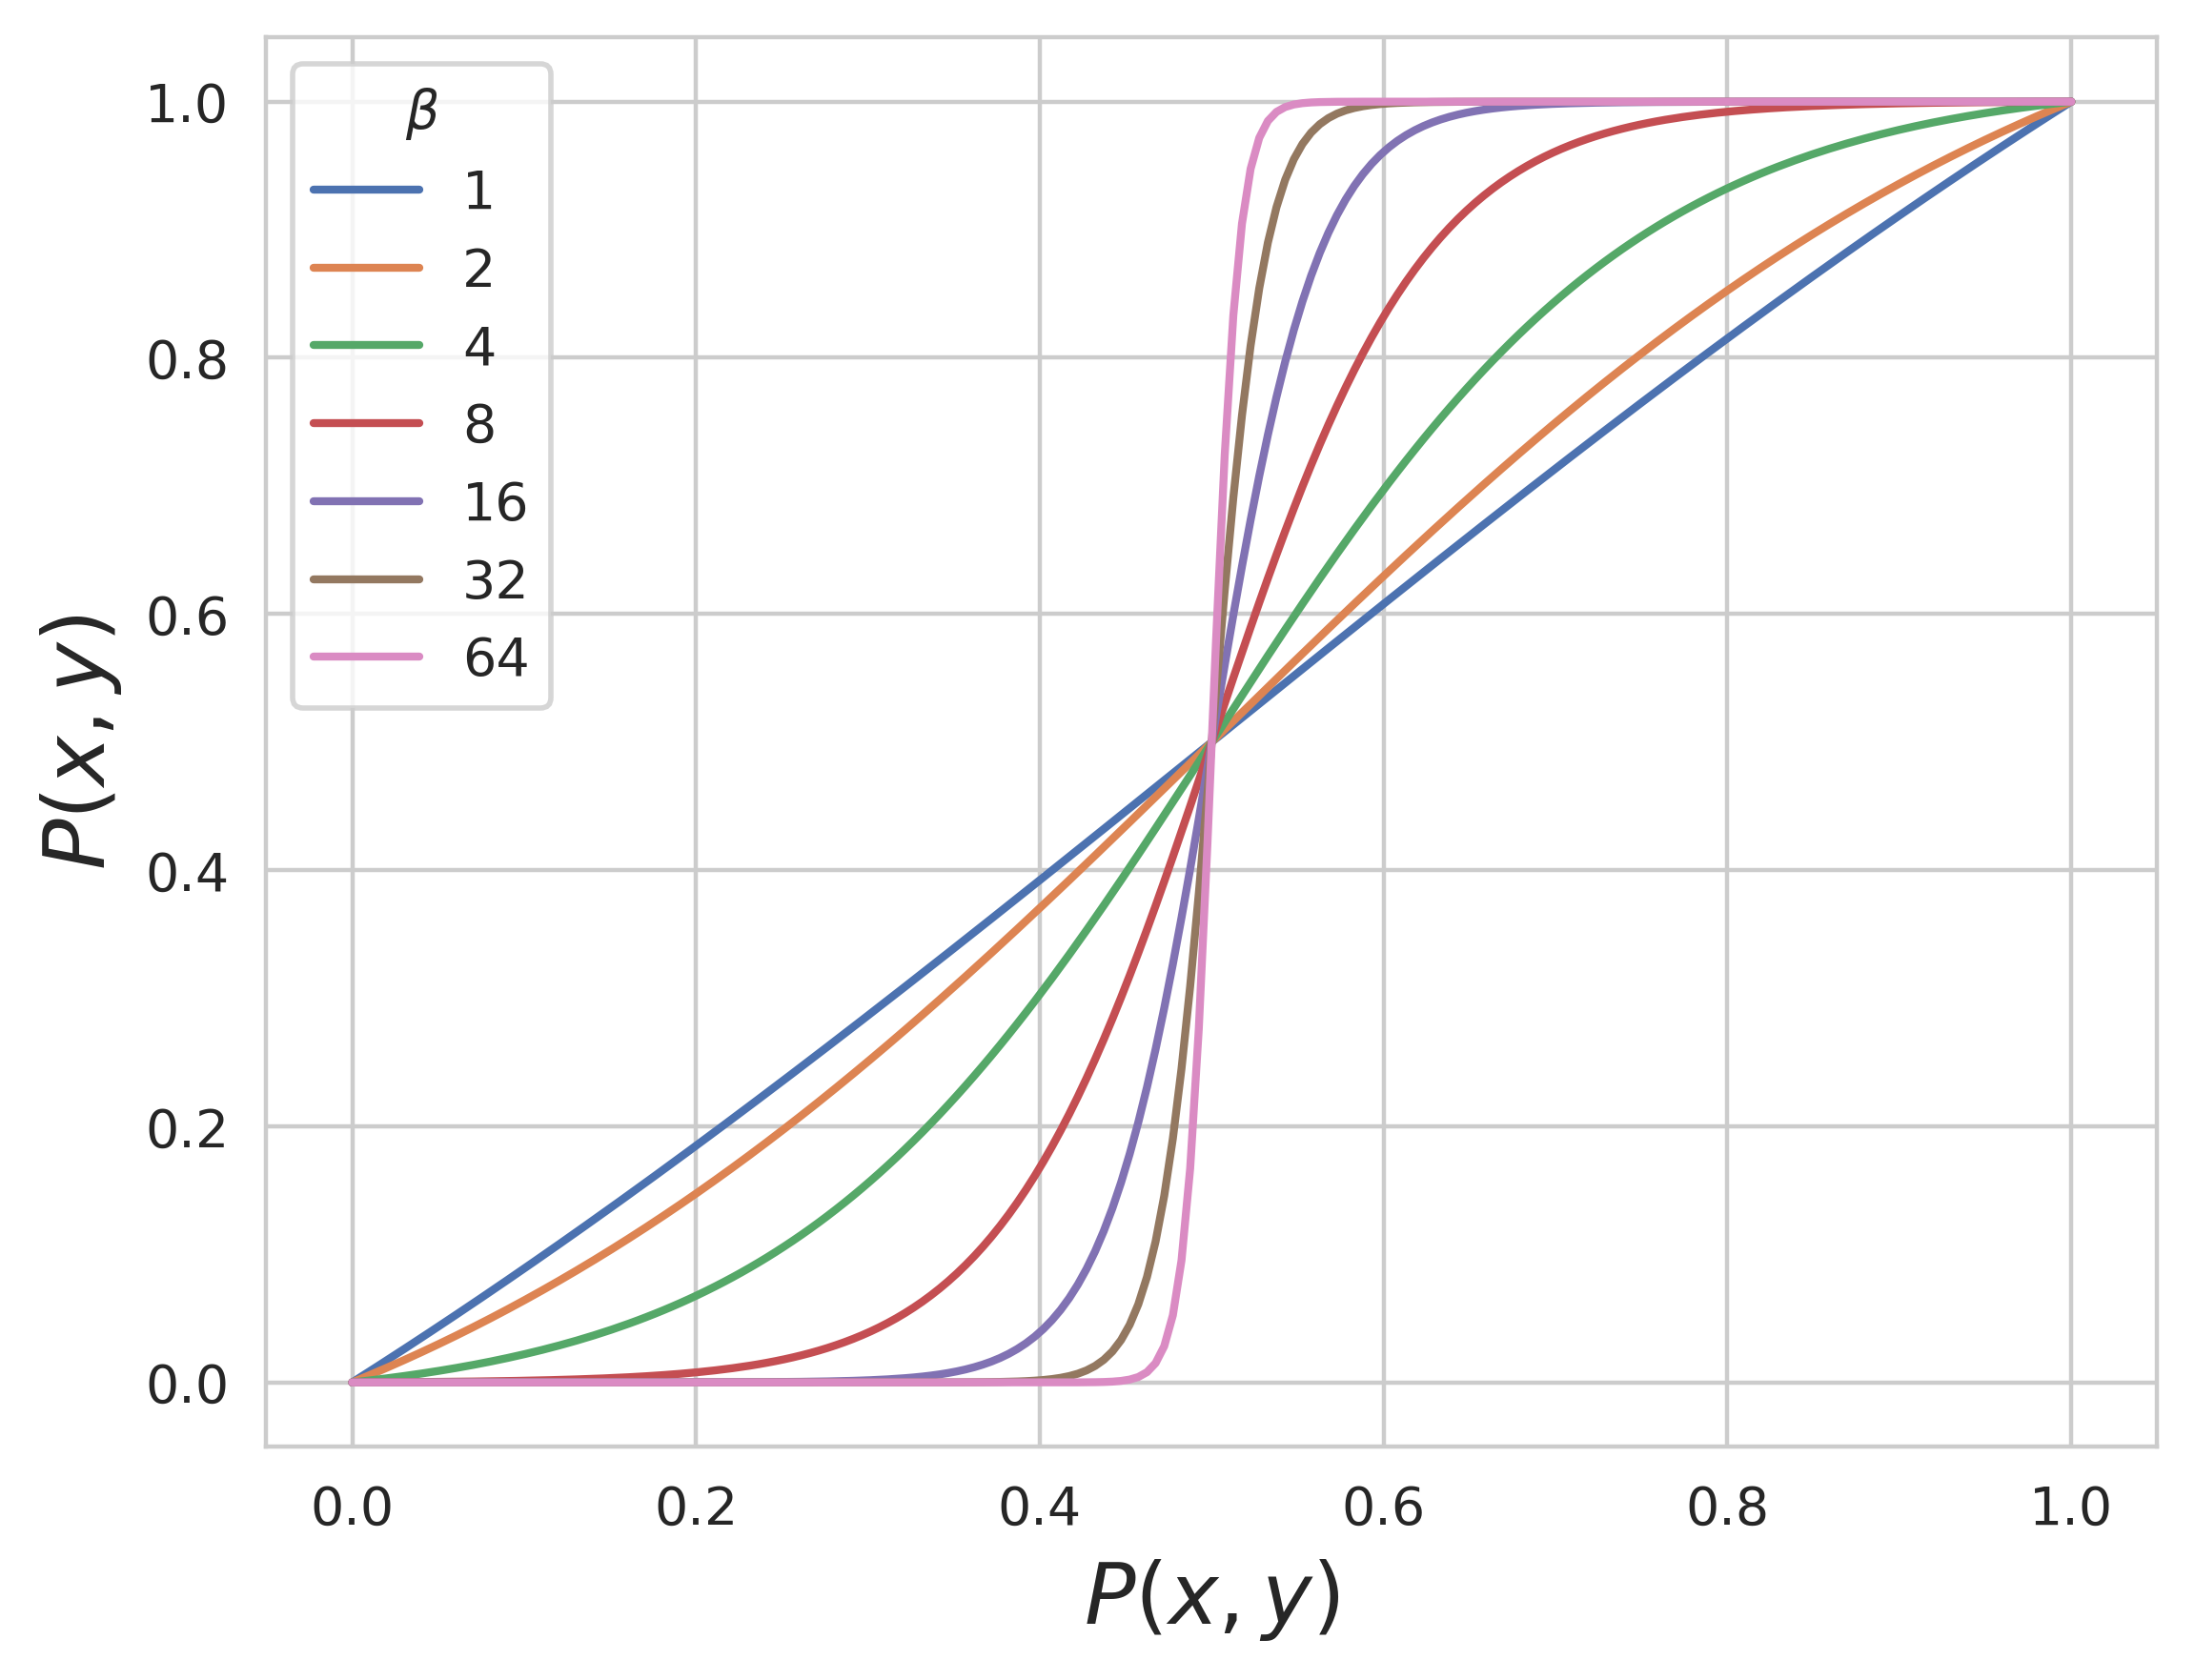
\includegraphics[scale=0.8]{image/theory/discretization.png}
      \caption{Función de discretización con $\eta = 0.5$ y distintos valores
      de $\beta$.}
      \label{fig:discretization}
    \end{figure}

\leonidas{TODO: Agregar una descripción detallada sobre las siguientes ecuaciones.}

\begin{equation}
  \widetilde{\boldsymbol{P}}(x, y) = \frac{\displaystyle\sum_{(x', y') \in B_{r_f}(x, y)} w_{x, y}(x', y')
  A(x', y')p_{x', y'}}
  {\displaystyle\sum_{(x', y') \in B_{r_f}(x, y)} w_{x, y}(x', y') A(x', y')},
  \label{eq:densityfilter}
\end{equation}

\begin{equation}
  w_{x, y}(x', y') = max(0, r_f - dis(x, y, x', y'))
  \label{eq:hatbased}
\end{equation}

\begin{equation}
  dis(x, y, x', y') = |x-x'|*psize_y+|y-y'|*psize_x
  \label{eq:distance}
\end{equation}

\begin{equation}
  \frac{\partial\widetilde{\boldsymbol{P}}(x, y)}{\partial \boldsymbol{P}(x^{*}, y^{*})} = \frac{w_{x, y}(x^{*},
  y^{*})A(x^{*}, y^{*})}
  {\displaystyle\sum_{(x', y') \in B_{r_f}(x, y)} w_{x, y}(x', y') A(x', y')},
  \label{eq:densityfiltergrad}
\end{equation}

\begin{equation}
  \frac{\partial\widetilde{\widetilde{\boldsymbol{P}}}(x, y)}{\partial \widetilde{\boldsymbol{P}}(x, y)} =
  \frac{(1 - \tanh^2 (\beta \times (\widetilde{p}_{x, y} - \eta)) \beta)}
       {\tanh (\beta \times \eta) + \tanh (\beta \times (1 - \eta))},
  \label{eq:projecition-grad}
\end{equation}

\begin{equation}
  \frac{\partial f_{obj}}{\partial \boldsymbol{P}(x, y)} = \displaystyle\sum_{(x', y') \in B_{r_f}(x, y)}
  \frac{\partial f_{obj}}{\partial \widetilde{\widetilde{\boldsymbol{P}}}(x', y')}
  \frac{\partial \widetilde{\widetilde{\boldsymbol{P}}}(x', y')}{\partial \widetilde{\boldsymbol{P}}(x', y')}
   \frac{\partial \widetilde{\boldsymbol{P}}(x', y')}{\partial \boldsymbol{P}(x, y)}
  \label{eq:fobjgrad}
\end{equation}

%\section{Preparación para fabricación}

%\subsection{Formato GDSII}

%Para poder fabricar nuestros diseños necesitamos representarlos en formato GDSII.
%En este formato se especifica los polígonos que representan a nuestro dispositivo.
%Independientemente de la parametrización utilizada, mediante la simulación con SPINS o MEEP se puede obtener los puntos asociados al contorno del dispositivo.
%Así, utilizando lo anterior se construye los polígonos \citep{Bogaerts2018}.

%\leonidas{Hablar en más detalle de esto y acompañarlo con una imagen de conversión de una curva al formato GDSII similar al paper de Lukas}

%\subsection{Simulación de errores}

%\leonidas{Escribir las fórmulas de dilatación y contracción de Hammond2020. Hacer un link con el método de los 9 puntos.}
